\section{Руководство пользователя}

\subsection{Назначение программы}

Разработанная программа реализует алгоритм сжатия изображений, повторяющий основные этапы стандарта JPEG. 
В отличие от оригинального алгоритма, на этапе энтропийного кодирования используется метод RLE (Run-Length Encoding) 
вместо кодирования по Хаффману. 
% Это позволяет упростить реализацию, сохранив при этом все основные свойства алгоритма JPEG.

% Программа предназначена для демонстрации полного цикла кодирования и декодирования изображения:

% \begin{itemize}
%     \item переход от $\textbf{RGB}$ к $\textbf{YCbCr}$
%     \item разбиение на блоки $8 \times 8$
%     \item дискретное косинус-преобразование (DCT)
%     \item квантование
%     \item последовательное сканирование (зигзаг)
%     \item кодирование RLE
%     \item обратные преобразования (IDCT и т. д.)
%     \item восстановление RGB-изображения

% \end{itemize}

% %%%%%%%%%%%%%%%%%%%%%%%%%%%%%%%%%%%%%%%%%%%%%%%%
% \subsection{Интерфейс программы}

% На рисунке 4.1 представлено главное окно приложения.

% \begin{figure}[h!]
%     \centering
%     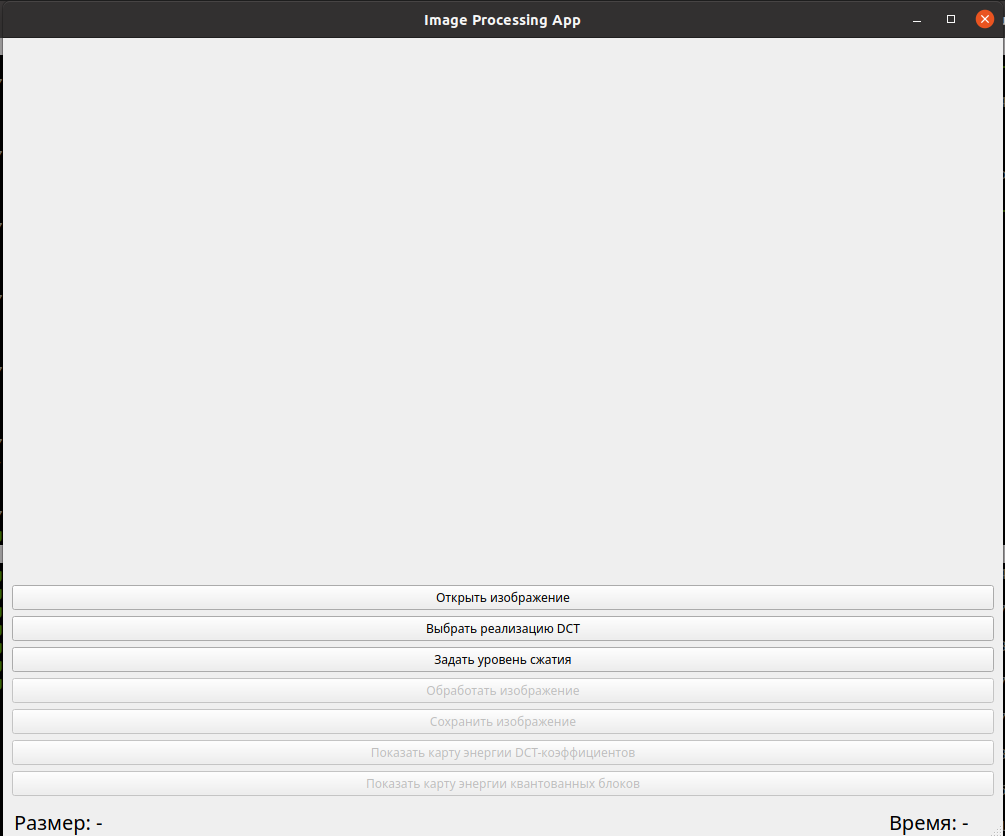
\includegraphics[width=0.7\textwidth]{/home/evgen/Coursework/app/diplom/images/interface.png}
%     \caption{Главное окно приложения.}
%     \label{fig:interface}
% \end{figure}
